\section{What does the network geometry establish?}

\subsection{Absolute rank, layer width, and an architecture control}

Absolute participation rank falls with depth, but hidden width also contracts from 128 to 64 to 32. The archived raw-centered medians are 20.251, 14.669, and 9.048 (Table~\ref{tab:geometry}). Dividing by width gives 15.8\%, 22.9\%, and 28.3\%, respectively. Thus the absolute decline does not show increasing concentration relative to the available coordinates. Feature z-scoring and row-$L_2$ normalization retain the absolute ordering, but cannot remove the architecture comparison by themselves.

A bounded supplementary control compares the 30 frozen trained networks with five untrained networks on exactly the same 384 securities in each of the 120 development months. Architecture, activation functions, input preprocessing, and seed identifiers match; the untrained hidden weights for a seed are shared across all six output dimensions rather than counted as six independent random networks. These are fresh draws under the recorded control runtime, not a recovery of the exact historical initialization tensors. The design was fixed before its execution, after the earlier manuscript and diagnostics were available.

The control separates two observations (Figure~\ref{fig:geometry-dashboard}). Random networks already have falling mean absolute ranks: 20.435, 15.253, and 10.399. Trained means are 20.318, 14.114, and 8.691. Training is associated with additional concentration, especially in the last two layers. The primary final-layer mean rank/width difference is $-5.340$ percentage points, with a paired 95\% interval of $[-7.737,-3.359]$. It uses 1,000 common twelve-month circular-block draws with paired seed resampling, retaining every $K$ within its seed. The interval is conditional on the archived networks and sample; five initializations limit generalization. The sign supports training-associated concentration beyond this random-network benchmark, not identification of a pricing dimension.

\begin{widetable}[!tbp]
\centering
\begin{minipage}{\textwidth}
\caption{Trained and random-network concentration on matched inputs}
\label{tab:architecture-control}
\footnotesize
\setlength{\tabcolsep}{4pt}
\renewcommand{\arraystretch}{1.16}
\begin{tabular*}{\linewidth}{@{\extracolsep{\fill}}crrrrr@{}}
\toprule
Layer & Width & Trained PR & Random PR & Gap / width (pp) & 95\% interval \\
\midrule
\multicolumn{6}{@{}l}{\textit{A. Raw centered}} \\[2pt]
H1 & 128 & 20.318 & 20.435 & -0.092 & [-0.214, 0.063] \\
H2 & 64 & 14.114 & 15.253 & -1.780 & [-2.596, -1.059] \\
H3 & 32 & 8.691 & 10.399 & -5.340 & [-7.737, -3.359] \\
\addlinespace[4pt]
\multicolumn{6}{@{}l}{\textit{B. Feature z-score}} \\[2pt]
H1 & 128 & 23.057 & 23.138 & -0.064 & [-0.175, 0.092] \\
H2 & 64 & 16.204 & 17.219 & -1.587 & [-2.229, -1.014] \\
H3 & 32 & 10.241 & 11.755 & -4.729 & [-6.667, -3.041] \\
\addlinespace[4pt]
\multicolumn{6}{@{}l}{\textit{C. Row-$L_2$}} \\[2pt]
H1 & 128 & 21.131 & 21.270 & -0.108 & [-0.217, 0.028] \\
H2 & 64 & 14.926 & 15.950 & -1.600 & [-2.412, -0.865] \\
H3 & 32 & 8.793 & 10.448 & -5.170 & [-7.412, -3.320] \\
\bottomrule
\end{tabular*}
\par\vspace{4pt}
{\footnotesize\raggedright\textit{Notes:} PR denotes participation rank. Entries are means, unlike the archived medians in Table~\ref{tab:geometry}. Width-normalized gaps are trained minus random. The primary endpoint is raw-centered H3; all other rows are descriptive. The 1,000 draws resample common twelve-month circular blocks and five paired seed clusters. Random hidden weights are shared across all six $K$ values. Intervals are pointwise and conditional on the archived sample and trained weights. This control was designed after the earlier study; it does not retune the economic-function probe.\par}
\end{minipage}
\end{widetable}


\begin{widetable}[!tbp]
\centering
\begin{minipage}{\textwidth}
\caption{Layerwise representation geometry under three normalization rules}
\label{tab:geometry}
\footnotesize
\setlength{\tabcolsep}{4pt}
\renewcommand{\arraystretch}{1.16}
\begin{tabular*}{\linewidth}{@{\extracolsep{\fill}}lrrrrrrr@{}}
\toprule
Layer & Participation & Entropy & PCA95 & TWO-NN & LB ($k=20$) & Tangent angle & Drift \\
 & rank & rank & rank & dimension & dimension & (radians) & (rank 5) \\
\midrule
\multicolumn{8}{@{}l}{\textit{A. Raw centering}} \\[2pt]
Hidden 1 & 20.251 & 35.855 & 50 & 15.477 & 13.835 & 1.493 & 0.987 \\
Hidden 2 & 14.669 & 23.760 & 32 & 14.072 & 12.054 & 1.474 & 0.862 \\
Hidden 3 & 9.048 & 13.839 & 18 & 11.814 & 9.757 & 1.437 & 0.670 \\
\addlinespace[5pt]
\multicolumn{8}{@{}l}{\textit{B. Feature z-score}} \\[2pt]
Hidden 1 & 22.989 & 38.444 & 51 & 15.750 & 14.186 & 1.494 & 0.942 \\
Hidden 2 & 16.538 & 25.430 & 32 & 14.237 & 12.399 & 1.477 & 0.890 \\
Hidden 3 & 10.476 & 15.097 & 18 & 11.990 & 10.058 & 1.429 & 0.661 \\
\addlinespace[5pt]
\multicolumn{8}{@{}l}{\textit{C. Row-$L_2$ normalization}} \\[2pt]
Hidden 1 & 21.168 & 36.728 & 50 & -- & -- & -- & 0.948 \\
Hidden 2 & 15.479 & 24.609 & 32 & -- & -- & -- & 0.856 \\
Hidden 3 & 9.105 & 13.903 & 18 & -- & -- & -- & 0.661 \\
\bottomrule
\end{tabular*}
\par\vspace{4pt}
{\footnotesize\raggedright\textit{Notes:} Entries are archived medians for 30 frozen networks and 120 development months. Spectral summaries use 3,600 observations per group; drift uses 3,570 adjacent-month pairs. Neighbor dimensions and tangent angles use only 300 observations per raw/z-score group (ten sampled months). LB is the Levina--Bickel estimator. Dashes denote diagnostics not computed under row normalization, not zero values. The numerical-collapse rate is zero; it is not a classification neural-collapse test. The two adjacent-layer CKA medians are 0.875 and 0.848. These are descriptive, finite-scale diagnostics; the separate economic-function test is reported in Figure~\ref{fig:evidence-ladder} and Section~\ref{sec:function-gate}.\par}
\end{minipage}
\end{widetable}


Independent synthetic calibration precedes the empirical estimates. The first calibration failed two of six gates because a fixed tangent-space rank could not distinguish curved from flat manifolds and the scale-artifact design did not match the z-score estimand. Those failures were retained. A corrected, frozen calibration chose local rank adaptively and aligned the scale design with the estimand; it passed plane dimensions 3 and 8, curvature, collapse, scale-artifact, and full-rank anisotropy gates. This supports use of the estimators as directional diagnostics, not as an oracle for unique intrinsic dimension.

The collapse rate is zero. The final layer's leading-eigenvalue share is 0.232 and its PCA90 and PCA95 dimensions are 14 and 18. Hence the pattern is anisotropic concentration rather than a representation converging to a constant or a one-dimensional line. Z-scoring increases final-layer participation rank by 1.427, or 15.8\%, which confirms some scale influence but remains far below the frozen 50\% artifact threshold.

\subsection{Concentration is not evidence of a smooth pricing manifold}

The term ``manifold'' suggests more than a low effective rank. It suggests that observations lie near a smooth lower-dimensional object whose local tangent spaces vary coherently. The finite-scale tangent-angle diagnostic is insufficient to establish that interpretation. Its median declines from 1.493 to 1.437 radians rather than increasing with depth. Values near a right angle indicate that local and larger-scale tangent estimates are not tightly aligned. The representation is concentrated, but the evidence does not establish a unique smooth manifold.

Adjacent-layer CKA medians are 0.875 for hidden 1 versus hidden 2 and 0.848 for hidden 2 versus hidden 3. Layers retain much of the same cross-sectional structure while reorganizing it. Rank-five monthly Grassmann drift falls from 0.987 to 0.862 and 0.670 across layers. Deeper principal subspaces are more stable over adjacent months even though they are not fixed.

High-volatility months have a final-layer raw participation rank only 0.165 above other months. The small association does not identify a volatility-driven state transition. It also illustrates why a geometrically stable subspace and a stable pricing function are different claims: the subspace can move less while the output weights or realized price of risk change materially.

\subsection{The prespecified economic-function gate fails}
\label{sec:function-gate}

The separate economic-function criterion is not met. The architecture control does not change this previously specified test or its endpoint. Figure~\ref{fig:evidence-ladder} displays the model-level prediction errors. The primary probe predicts each model's development-period HJ loss from final-layer geometry after controlling for nominal factor count. Validation leaves out one seed at a time so that a seed-specific geometry--performance relation cannot be evaluated on the same seed used to fit it. Adding geometry reduces RMSE from 0.106 to 0.102, an improvement of 3.915\%. This is below the prespecified 5\% threshold, and the within-factor-count permutation $p$-value is 0.149. The within-factor-count Pearson correlation is $-0.296$.

The secondary factor-Sharpe endpoint has permutation $p=0.041$ but improves RMSE by only 1.211\%. It cannot replace the failed HJ endpoint. Searching another layer, normalization, state split, or economic outcome after seeing the result would convert a prespecified test into an unbounded geometry search. The analysis therefore stops at the planned gate.

\begin{widefigure}[!tbp]
\centering
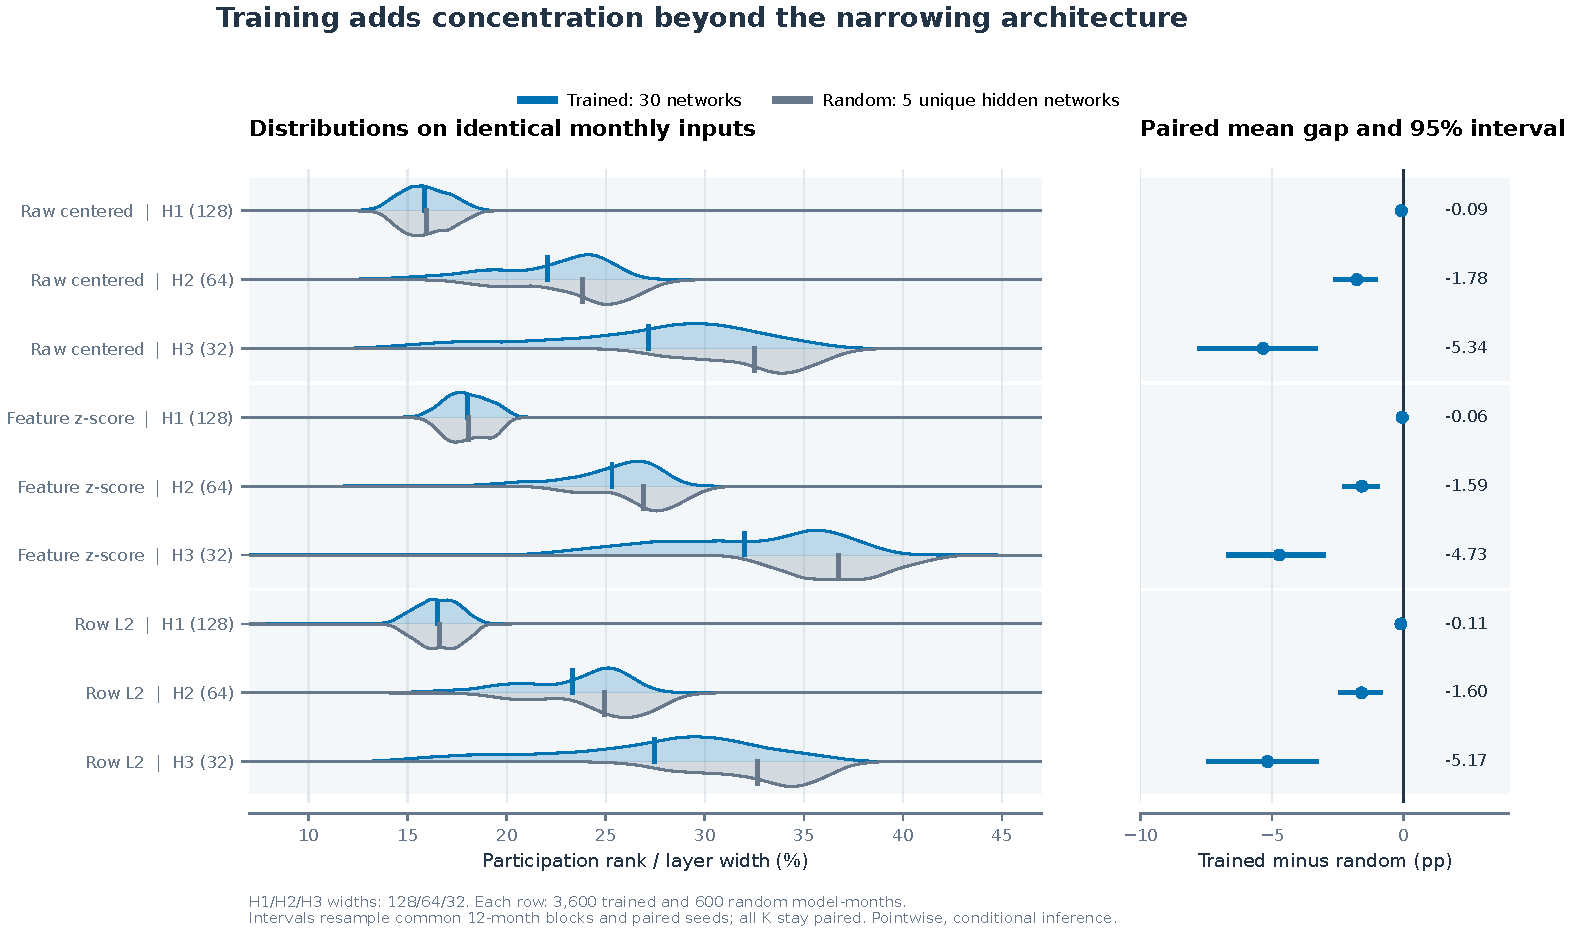
\includegraphics[width=0.98\textwidth]{figure_07_geometry_function.pdf}
\caption{Architecture-matched representation control. Each row compares participation rank divided by layer width for the original diagnostic networks and matched random networks on the same monthly inputs. The later conditional-autoencoder models are not included. There are 3,600 trained and 600 unique random observations per row; random hidden weights are shared across $K$. Markers show means. The aligned right-hand intervals report trained-minus-random mean differences in percentage points under paired twelve-month block and seed resampling. These are pointwise descriptive intervals. Absolute rank falls even in random networks; the training-associated gap is a separate comparison from the failed economic-function probe in Figure~\ref{fig:evidence-ladder}.}
\label{fig:geometry-dashboard}
\end{widefigure}

The result clarifies what high-dimensional networks may be doing. They map 86 characteristics and 86 missingness indicators into anisotropic hidden coordinates. Absolute rank declines as layers narrow, and training adds concentration relative to matched random networks. Rank-five subspaces also move less between adjacent months in deeper layers. But concentration does not reveal the number of priced shocks. It may reflect denoising, redundancy removal, saturation, common firm-characteristic structure, or an architecture-induced spectral bias. For the proposed incremental pricing interpretation, the geometry must predict pricing moments, SDF performance, or exposure spans beyond what nominal factor count already explains. The prespecified probe does not provide that incremental evidence here.

\subsection{Connecting geometric and economic compression}

The empirical pieces are consistent without being identical. The hidden representation concentrates to an effective rank near nine, while endpoint pricing choices range among one, two, four, five, and eight depending on data and loss. There is no contradiction: effective rank counts active variation in hidden activations, whereas pricing dimension counts directions needed to reduce a particular set of Euler errors. Some active hidden directions can support nonlinear sorting without carrying distinct risk prices. Some weak priced directions can have little activation variance and still matter under an HJ geometry or for a targeted asset family.

The economic direction of compression provides the bridge. Development decompositions show that a dominant common payoff direction explains part of the geometry contrast. The hidden-state evidence shows a broad anisotropic representation rather than a literal one-factor code. One interpretation is that a few common directions contain much of the variation, while additional directions may refine relative pricing. These diagnostics do not identify that hierarchy within individual hidden units. Which refinement counts as necessary depends on asset spanning, the metric, measurement, and the historical risk-price configuration.

These distinctions motivate reporting a spectrum, descriptive loss gaps or a stated tolerance set, and economic labels only for directions supported by the design. In the original diagnostics, the common market-direction point estimates retain a sign more consistently than the exact validation minimum; their wide intervals limit a stronger comparison. That is the sense in which compression can be economically interpretable without being a stable law of exact dimension.
